\chapter{提案システム\label{sec:proposal_system}}
\thispagestyle{plain}

本章では,本研究で提案するシステムについて述べる.

\section{概要}

本研究で提案するシステムの目的は,作業通話における作業嗜好の透明性の向上と,作業通話への募集・参加における心理的負担の低下である.

本システムの構成を図\ref{fig:matching_system_big_arrow}に示す.
本システムは,対話雰囲気推定モジュールとそれを用いたマッチング支援モジュールから構築される.
図\ref{fig:matching_system_big_arrow}において,データベースを境にそれまでのフローが対話雰囲気推定モジュール,それ以降のフローがマッチング支援モジュールである.
本システムは,はじめに対話雰囲気推定モジュールで作業通話の音声から対話雰囲気の推定及び,メタデータやアカウント情報の収集を行いデータベースに記録する.
続いて,それらのデータを基にマッチング支援モジュールでは二つの機能を提供する.
一つ目の機能は,ユーザの作業記録や作業傾向の可視化を行う機能である.
本機能では,それまでに集めたユーザ自身の作業嗜好を表す活動雰囲気のデータの統計値をはじめ,作業時間や発話量などの傾向を算出し表示する.
二つ目の機能は,ユーザの作業記録や作業傾向を基にした募集文の生成を行う機能である.
本機能では,参加者を募りたい作業通話の概要を入力することで,その概要と一つ目の機能で可視化された自身のデータを掲載された募集文(ツイート)を生成し投稿する.

\begin{figure}
    \centering
    \fbox{
        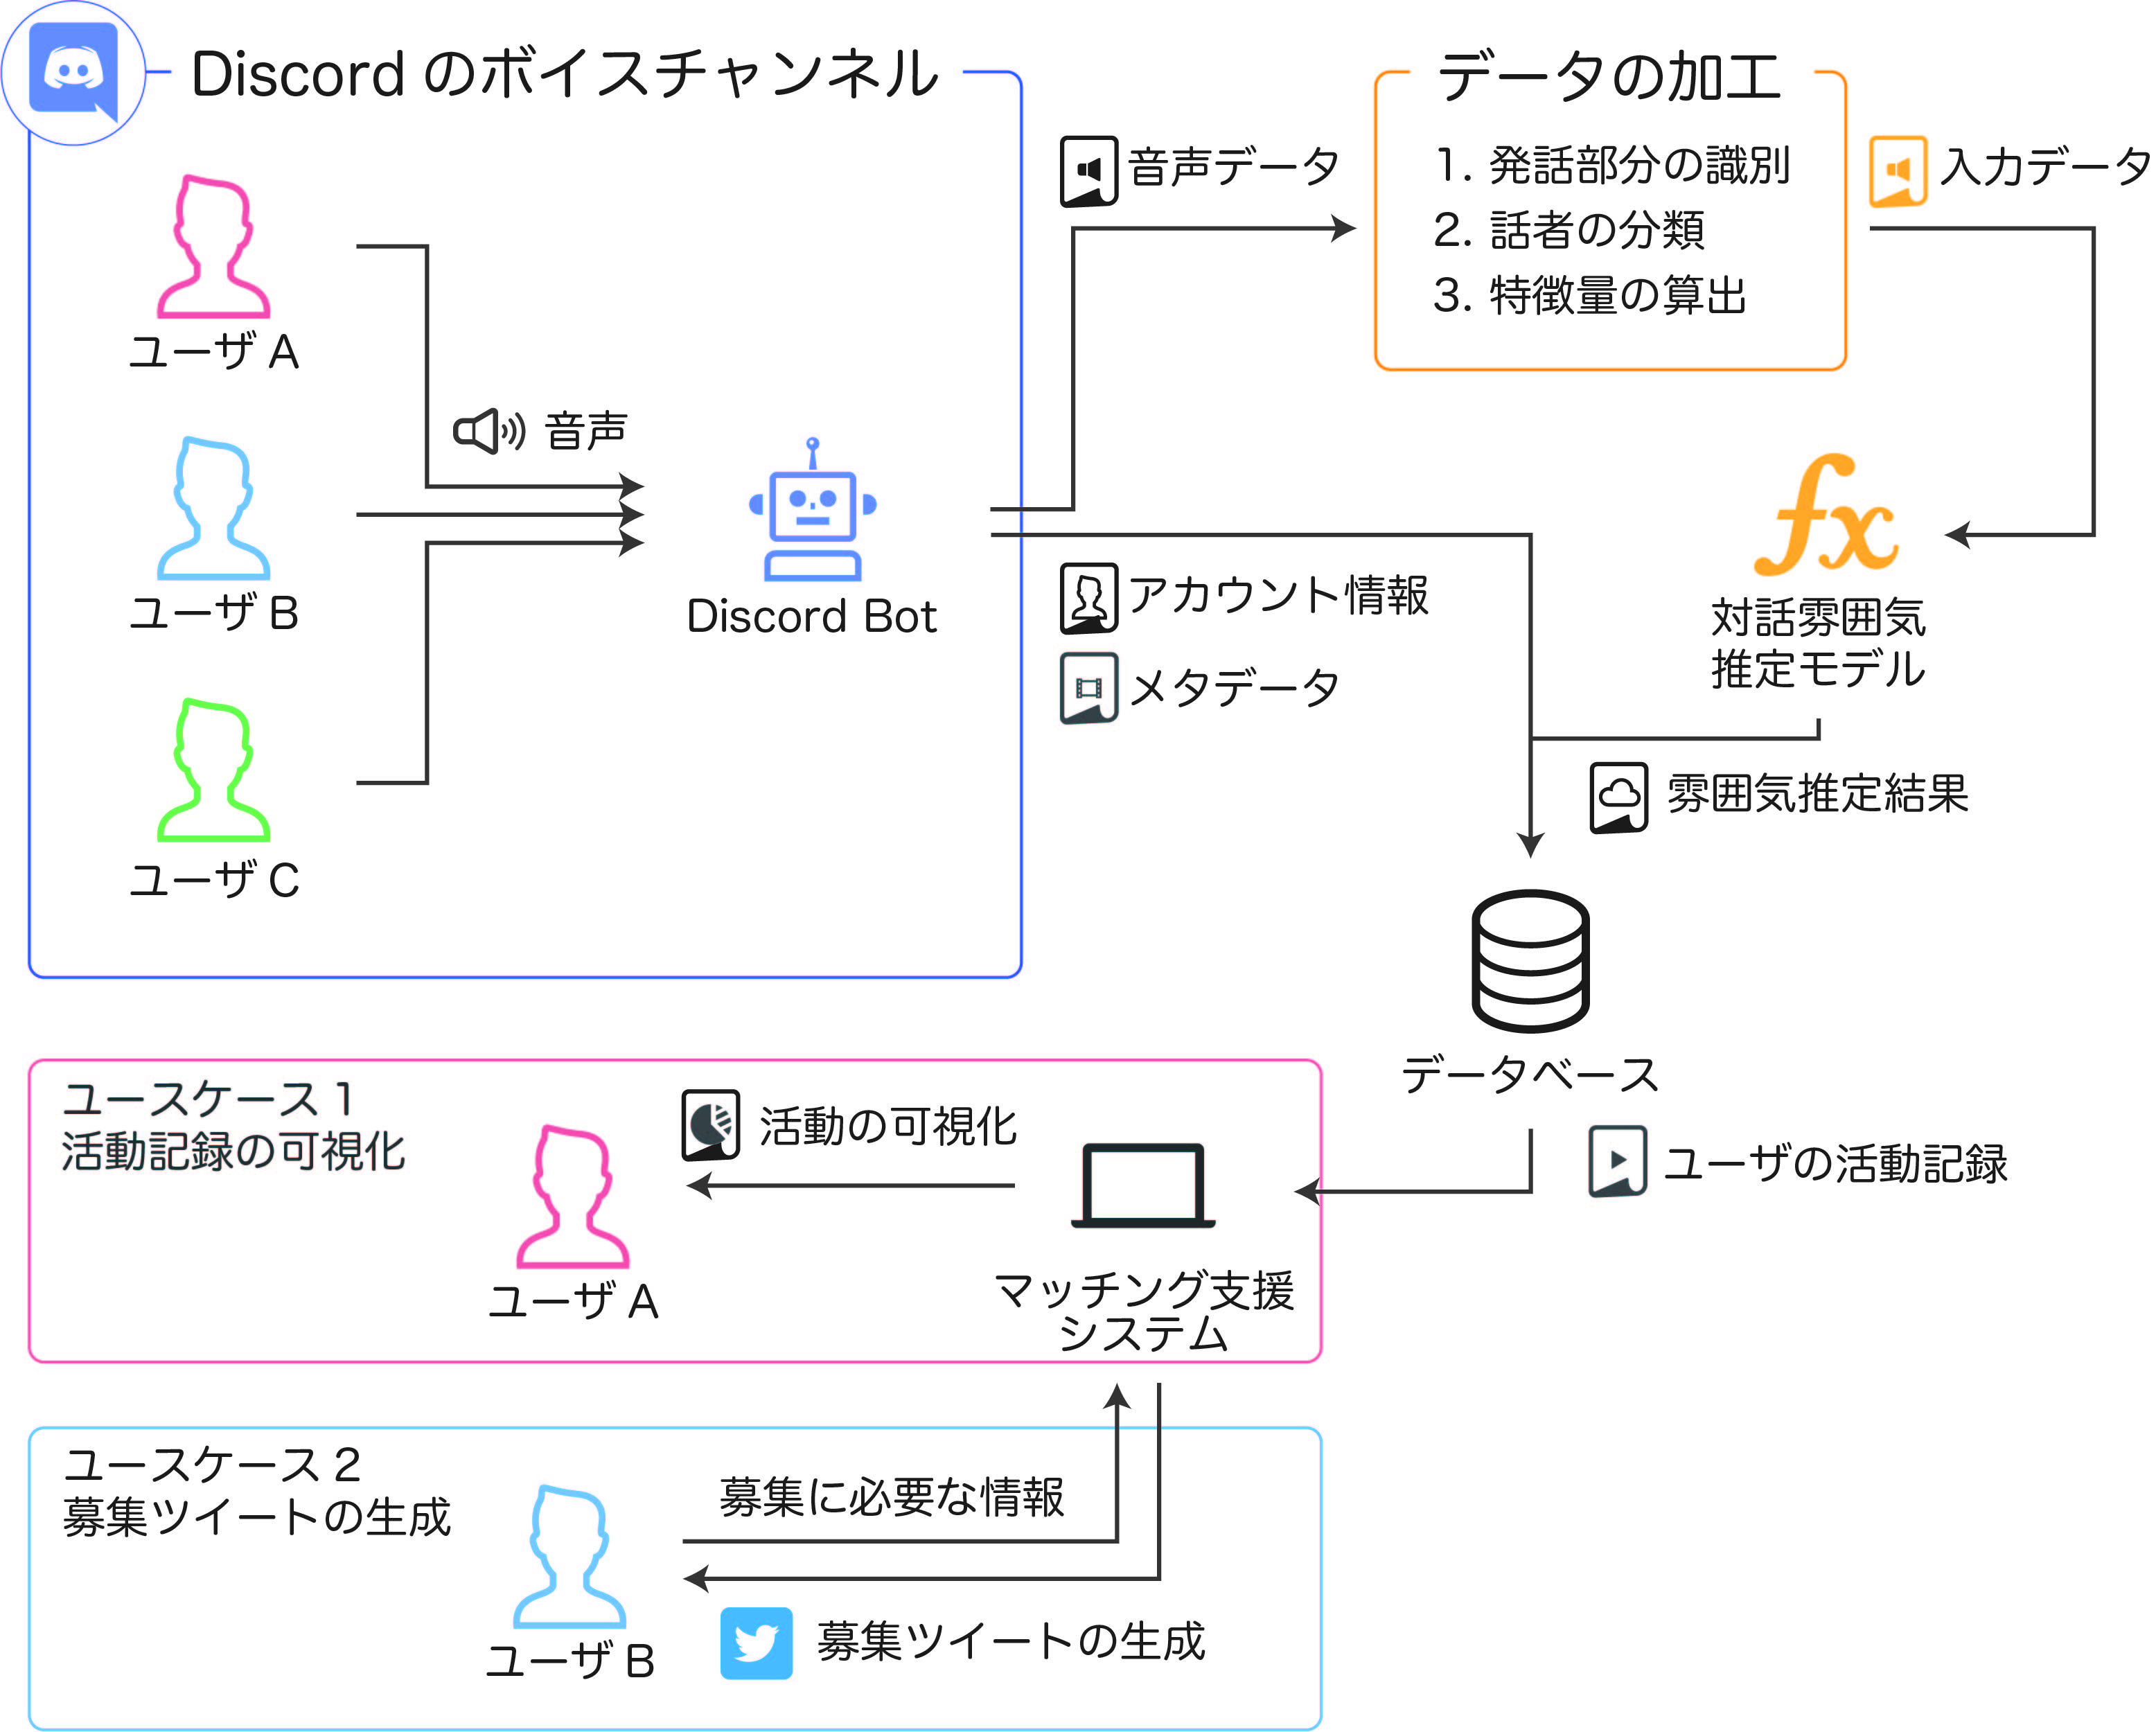
\includegraphics[width=0.7\textwidth]{figs/matching_system_big_arrow.jpg}
    }
    \caption{システムイメージ}
    \label{fig:matching_system_big_arrow}
\end{figure}

\section{対話雰囲気推定モジュール\label{node:estimation_module}}

本モジュールはDiscordで開催される作業通話を対象としており,作業通話の音声をBotによって収集し対話雰囲気の推定を行う.

\subsection{対話雰囲気推定モジュールで収集するデータ\label{item:estimation_module_collection_data}}

本モジュールは,対話雰囲気推定のために音声データの収集を行う.
その際には,第\ref{sec:related_researchs}章で述べた豊田らの手法を参考に,ユーザのプライバシーの担保や第\ref{sec:develop_estimation_model}章で述べる対話雰囲気推定モデルの構築における学習コストの低減を目的に限られた非言語情報のみを対象とする.
具体的には,どのユーザごとの発話時間情報(ユーザがいつどのくらいの時間発話を行ったかの情報)と作業通話のメタデータのみを用いる.
作業通話のメタデータとしては,参加者のユーザ情報,開催時間情報が収集対象である.
また,収集した発話時間情報は特徴量として変換され対話雰囲気推定モデルの入力データとして対話雰囲気の推定に利用する.

\subsection{対話雰囲気推定モジュールで推定する雰囲気\label{item:estimated_atmosphere}}

本モジュールで推定を行う対話雰囲気は「盛り上がり」,「真面目さ」,「明るさ」,「くつろぎ」の四つである(表\ref{tab:estimation_definition}).
本研究のそれぞれの定義について述べる.

「盛り上がり」は対話の活発性を表現する雰囲気を指す.
「盛り上がり」が肯定の状態,つまり盛り上がっている雰囲気とは参加者同士のコミュニケーションが頻繁に行われており,相互行為が活発に行われている状態を指す.
反対に,「盛り上がり」が否定の状態,盛り下がっている,沈んでいる雰囲気とは参加者同士の会話や相互行為が少ない状態を指す.

「真面目さ」は対話の生産性や参加者が対話に熱心に取り組んでいるかを表現する雰囲気を指す.
「真面目さ」が肯定の状態,つまり真面目な雰囲気とは参加者が作業や議題に集中しており,生産性が高い状態を指す.
反対に,「真面目さ」が否定の状態,真面目でない,怠けている雰囲気とは参加者が雑談をしていたり,主目的とは別の言動を行なっている状態を指す.

「明るさ」は話題の内容や参加者の態度を表現する雰囲気を指す.
「明るさ」が肯定の状態,つまり明るい雰囲気とは話題がポジティブで,参加者が興奮している状態を指す.
反対に,「明るさ」が否定の状態,暗い,落ち着いた雰囲気とは話題がネガティブで,参加者が物事に対して否定的な状態を指す.

「くつろぎ」は参加への心理的安全性や対話への満足感を表現する雰囲気を指す.
「くつろぎ」が肯定の状態,つまりくつろいでいる雰囲気とは参加者同士の心理的安全性が高く,リラックスして参加できている状態を指す.
反対に,「くつろぎ」が否定の状態,気遣っている,緊張している雰囲気とは参加者がお互いの距離感や接し方がわからない状態や,物事に注視して集中している状態を指す.

これらの対話雰囲気は本研究独自で定義したものであり,参考にしている豊田らの定義した雰囲気とは異なる.
これは,豊田らは対面で行われる二者間の対話を対象としていることに対して,本研究では遠隔で行われる複数名での作業通話中の対話を対象としているためである.

これらの対話雰囲気の推定には機械学習を用いる.
具体的には対話雰囲気推定モデルを構築し,そのモデルによって入力された一つの対話における各雰囲気について肯定か否定の2値で推定を行う.
対話雰囲気推定モデルについては第\ref{sec:develop_estimation_model}章で詳細に述べる.

\begin{table}[t]
    \caption{推定を行う雰囲気}
    \centering
    \begin{tabular}{|l|l|l|l|}
        \hline
        名称 & 定義 & 肯定 & 否定 \\
        \hline\hline
        盛り上がり & 対話の活発性を表現 & 盛り上がっている & 沈んでいる \\
        \hline
        真面目さ & 対話の生産性や参加者が対話に & 真面目である & 怠けている \\
        & 熱心に取り組んでいるかを表現 & & \\
        \hline
        明るさ & 話題の内容や参加者の態度を表現 & 明るい & 暗い \\
        \hline
        くつろぎ  & 参加への心理的安全性や & くつろいでいる & 緊張している \\
        & 対話への満足感を表現 & & \\
        \hline
    \end{tabular}
    \label{tab:estimation_definition}
\end{table}

\subsection{対話雰囲気推定モジュールの利用方法}

対話雰囲気推定モジュールのユーザが操作を行う箇所はDiscord Botのみである.
本節ではDiscord Botの利用方法の想定を示す.
まず,Discord Botはユーザが作業通話を開催するサーバに招待されることで利用可能状態となる.
ユーザは作業通話を開始した際に開始用のコマンドをDiscord Botに対して入力することで録音を開始する.
また,ユーザは作業通話が終了した際に終了用のコマンドを入力.
終了用のコマンドを受信したDiscord Botは録音の停止と対話雰囲気の推定結果の出力をテキストチャンネル上に行う.
ユーザはDiscord Botにより出力された対話雰囲気の推定結果の確認や,主観的に正しいと感じた雰囲気への修正を行える.
それらのデータはデータベースに記録される.記録したデータは再び学習データとしてモデルの精度向上に利用されることを想定している.

\section{マッチング支援モジュール}

本モジュールは,第\ref{node:estimation_module}節のモジュールによってデータベースに記録されたデータを用いた二つのユースケースを想定した機能の実装をしている.

一つ目は,自身の活動記録や作業嗜好を客観的に確認したいというユースケースに向けた活動記録や作業嗜好の可視化機能である.
本機能は,ユーザの今まで開催した作業通話に関するデータを表示する(図\ref{fig:estimationgraph}).
表示する情報は,平均発話量,平均活動時間,一緒に活動する人,雰囲気それぞれについての傾向値である.
平均発話量の傾向値は,発話回数と発話時間を基に対象ユーザが無口であるか多弁であるかをスライダーで示す.
また,1分あたりの平均発話時間も併せて記載する.
平均活動時間の傾向値は,メタデータを基に平均活動時間長が短いか長いかをスライダーで示す.
また,作業通話を開催している時間帯の傾向についても併せて記載する.
一緒に活動する人の傾向値は,メタデータを基に作業通話を知人と初見どちらの人と開催することが多いかをスライダーで示す.
ここにおける知人とはDiscord上でフレンドになっているか,一度以上過去にともに作業通話を行なった記録がある人を指す.
雰囲気の傾向値とは盛り上がっている雰囲気の対話が多いことなどをレーダーチャートにて表現した値を示す.

\begin{figure}
    \centering
    \fbox{
        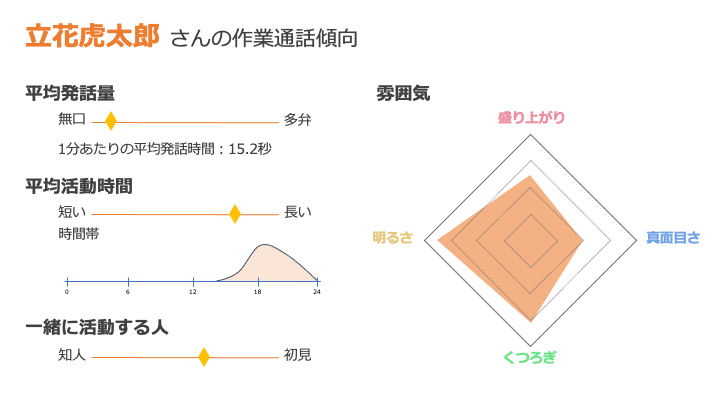
\includegraphics[width=0.7\textwidth]{figs/visualization.png}
    }
    \caption{作業嗜好の可視化イメージ}
    \label{fig:estimationgraph}
\end{figure}

二つ目は,効果的なSNS募集を行いたいというユースケースに向けた募集文(ツイート)の生成機能である.
本機能は,参加者を募りたい作業通話の概要を入力することで,その概要と一つ目の機能で可視化された自身のデータを掲載された募集文(ツイート)を生成し投稿する(図\ref{fig:tweet_image}).
本機能の対象は,Twitterで行われるSNS募集である.
本機能でユーザが入力する作業通話の概要情報は,作業内容,開催時間,募集人数の三つを想定している.
本機能は,一目で無縁ユーザ向けの募集文であることがわかることと,開催したい作業通話の概要がわかることによって明確で効率的な募集形態の実現を目指している.

\begin{figure}
    \centering
    \fbox{
        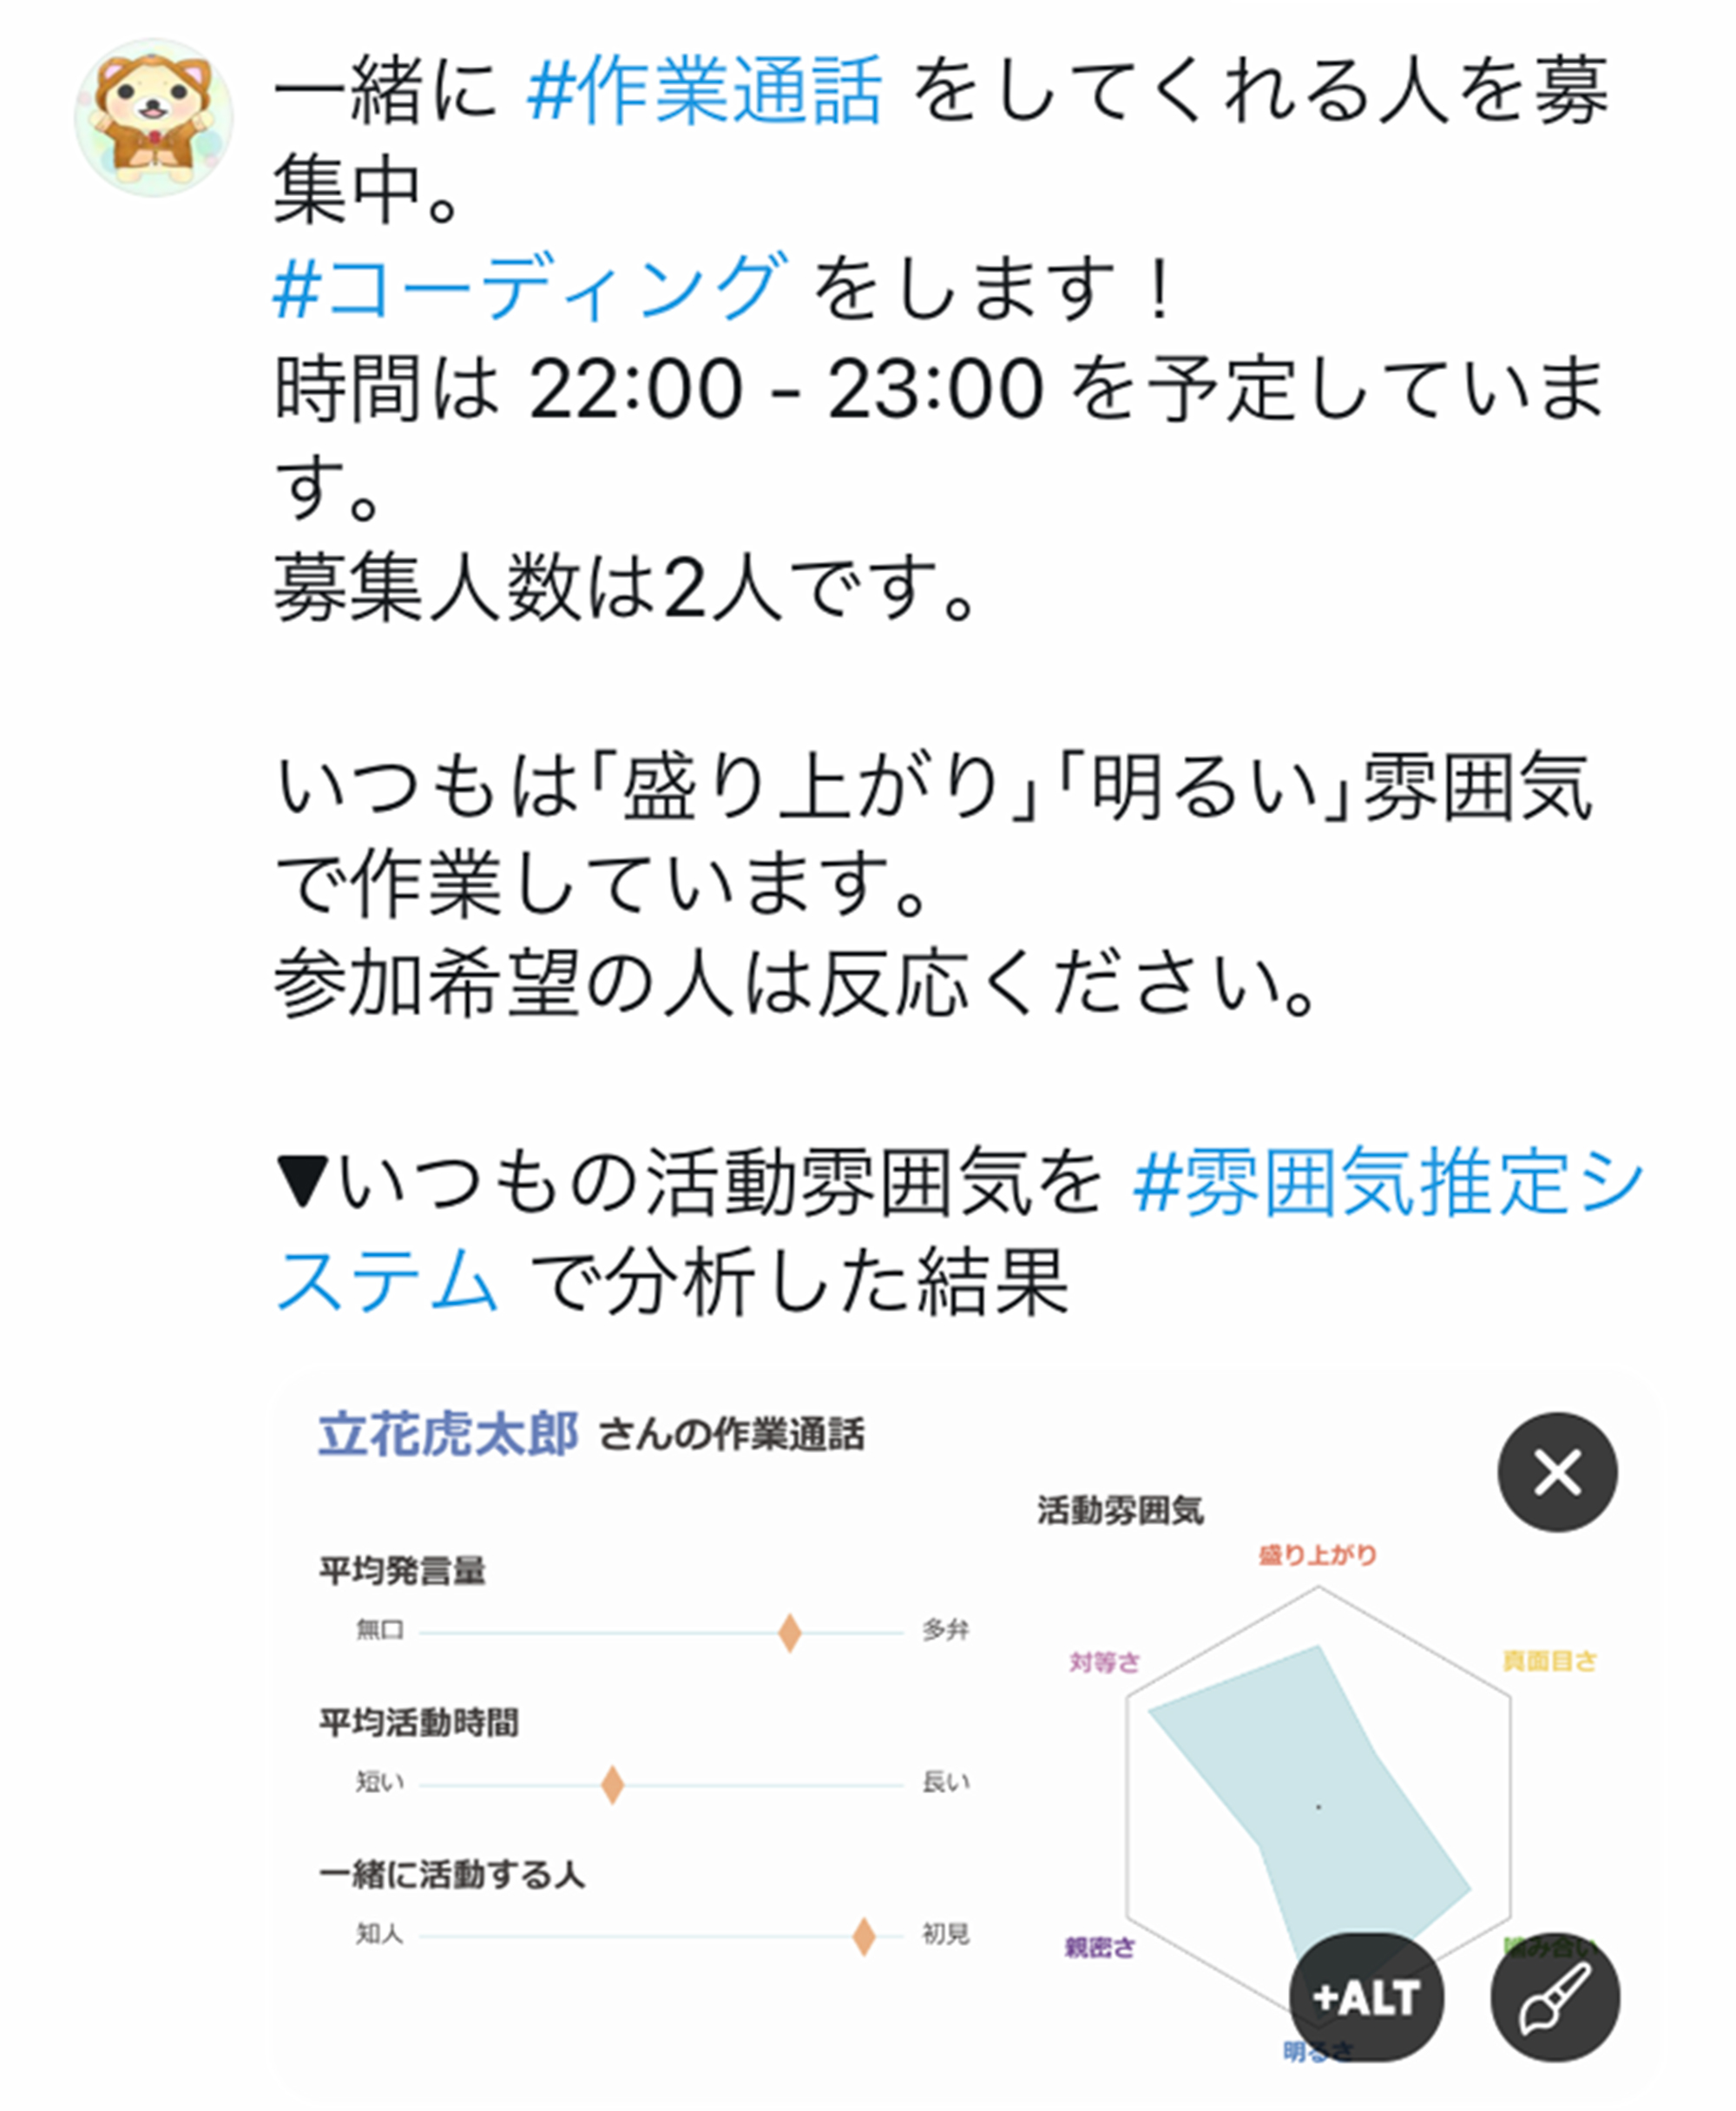
\includegraphics[width=0.7\textwidth]{figs/tweet_image.jpg}
    }
    \caption{生成する投稿のイメージ}
    \label{fig:tweet_image}
\end{figure}

将来的には,本モジュールを用いて作業嗜好の合うユーザの推薦等無縁ユーザとの繋がり形成の機会を増加させる機能の実装なども目指している.
結果として,SNS募集のデファクトスタンダードとなることでSNS募集の効率化と心理的負担の低下の実現を行えるモジュールを目指す.
